\documentclass[tikz]{standalone}

\usepackage{tikz}
\usetikzlibrary{automata}

\begin{document}

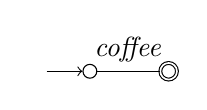
\begin{tikzpicture}
    \tikzstyle{every state}=[
        draw,
        shape=circle,
        inner sep=1pt,
        minimum size=5pt,
        final/.style={double,minimum size=6pt},
        initial text=]
 
    [->,auto,node distance=1.5cm]
    \renewcommand{\a}[1]{\textit{#1}}
    \node[state,initial] (a0) {}; 
    \node[state,final,right of=a0] (a1) {};
    \path (a0) edge node[above] {\a{coffee}} (a1);
\end{tikzpicture}
\end{document}